% #############################################################################
% This is Chapter 4
% !TEX root = ../main.tex
% #############################################################################
% Change the Name of the Chapter i the following line
\fancychapter{Architecture}
\cleardoublepage
% The following line allows to ref this chapter
\label{chap:arch}

The fundamental objective of this work is to develop a portable device,  which enables entities to establish secure channels of communication.
A solution was developed on a portable HSM, which secures communications between users, stores the owner's sensitive data, such as keys and documents, and performs all services critical to its security. This is an easy process for the owner, who does not need to concern himself with any setup or management, the system is accessible and ready to use when received.
This chapter presents an overview of the developed system, its services, the communications protocol and use cases, unconstrained by a specific physical device.

% -----------------------------------------------------
% -----------------------------------------------------
\section{Overview}\label{chap:arch:overview}

%% COMPONENTS INTRODUCTION %%
The system, pictured in Figure~\ref{fig:overview}, is composed of two main components: the physical device, responsible for all operations, and the application on the user's computer, which provides a straightforward interface to users.

\begin{figure}[h]
    \centering
    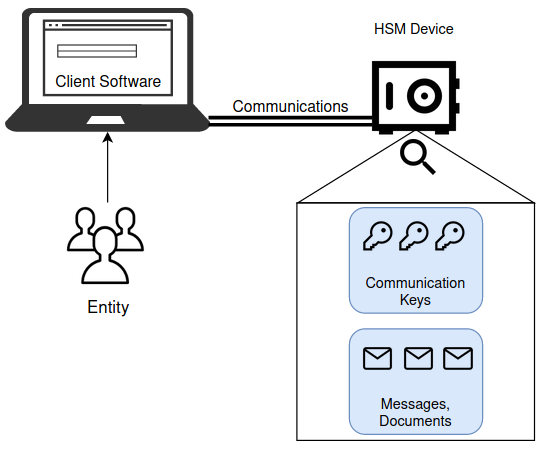
\includegraphics[width=0.7\textwidth]{./Images/overview.png}
    \caption{System Overview}
    \label{fig:overview}
\end{figure}

%% SYSTEM OVERVIEW %%
The user's computer running the software is connected to the device, through a physical connection, used to send and receive data and commands.
Using these tools, the user can signal the device to perform the desired services.
These services are implemented inside the device, which stores and manages keys, as well as other data.
If the device is misplaced or stolen, the stored keys and documents are not at risk of being extracted. The developed software and physical tamper measures ensure it.
Upon receiving their device, each user is only required to plugin it into a power socket, and to their computer using the appropriate cable. The system is ready to use, through the provided interface software.
%% SERIAL PORT COMMUNICATIONS INTRODUCTION %%
All data and commands will flow through a serial connection, between the interface software in the individual's computer and the physical box. A communication protocol which defines the communication rules is defined in the next section.
% Data is organized in fields, each field has a fixed number of bytes to hold a specific piece of data.
% The protocols are organized in transmissions. One transmission is two messages, one message from the computer to the device, and another in the reverse direction.
% The serial port connection transmits data one block at a time, each block contains a maximum of 16 bytes.

% -----------------------------------------------------
% -----------------------------------------------------
\section{Services Protocols}\label{chap:arch:services}

%% INTRODUCTION %%
This section describes the services and their communication protocol, between the computer application and the hardware device. Each service's goal, exchanged information and algorithms are also detailed.
Firstly it presents the authentication, then main services, divided in their objective, secure data exchange, digital signatures and new communications.
In the diagrams representing the protocols, consecutive pieces of data flowing in the same direction are separated in distinct messages for visual purposes only. In practice, the data is sent in one message, each in its own field with a defined number of bytes.

% -----------------------------------------------------
% \subsection{Initial State}\label{chap:arch:services:initial-state}

%% DEVICE STATE FROM FABRIC %%
The device will come from fabric configured and prepared with the necessary keys to secure communications.
Before acquiring the device, each entity can provide a list of entities with whom they wish to securely communicate. The device will then be delivered to each entity with the necessary keys. This allows owners to begin to communicate immediately, with no setup necessary.
Additionally, the device is delivered with the necessary functionality and keys, so all devices can establish secure communications with new entities. This provides the flexibility of secure data exchange with a new entity, without having to send the device back to the distributor, to be loaded with the necessary keys.

% -----------------------------------------------------
\subsection{Authentication}\label{chap:arch:services:auth}

All users need to be authenticated through a PIN number, in order to access the system operations. This way, each entity with multiple users can organically handle which users are authorized to access the device, by handing out the corresponding PIN number.
The device is delivered with a default PIN to the owner. It can be changed at any time by an authenticated user.
To authenticate himself to the device, the user sends the operation code, and PIN through the software, the device then compares it to the authentication number securely stored inside it, and receives an appropriate failure or success status. Once authenticated, the session will be unlocked, and the user gains access to all services.
The protocol to change the authentication PIN is exactly the same as the login, with the exception that the supplied PIN is the new PIN, which will overwrite the current. The user will receive an error status if it is not logged in.
% Figure~\ref{fig:protocol:login} depicts the login protocol.

% \begin{figure}[h!]
%         \centering
%         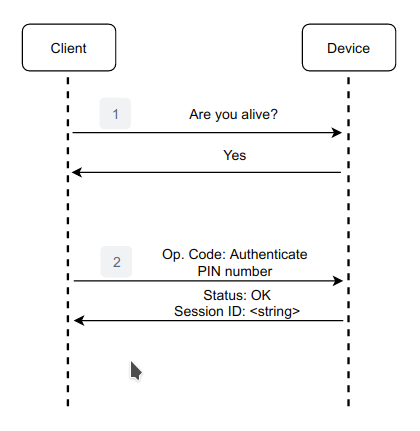
\includegraphics[width=0.50\textwidth]{./Images/authentication.png}
%         \caption{Login and PIN change communication protocol}
%         \label{fig:protocol:login}
% \end{figure}

% -----------------------------------------------------
\subsection{Secure Data Exchange}\label{chap:arch:services:data-exchange}

The secure data exchange service is responsible for securing communications between users. It grants confidentiality, integrity and authentication to communications.
The communication protocol, between the device and computer application, is illustrated in Figure~\ref{fig:protocol:data-exchange}, and consists of two transmissions.
\begin{figure}[h!]
	\centering
	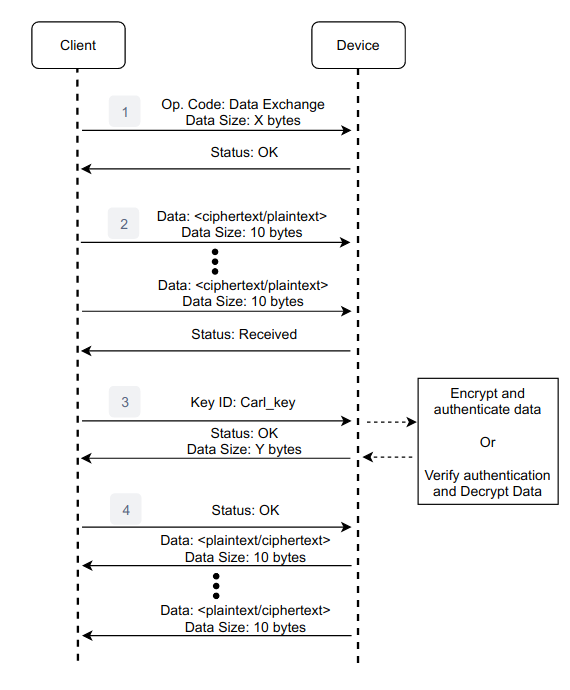
\includegraphics[width=0.60\textwidth]{./Images/data-exchange.png}
	\caption{Communication protocol for data ciphering and authentication in the HSM with internal keys}
	\label{fig:protocol:data-exchange}
\end{figure}

The first transmission is started by the user, by sending the operation code and key ID, which identifies the internal symmetric key used to encrypt and authenticate.
The device returns a status message. If the key ID was invalid or the user is not authenticated, it is an error.
In the second transmission, the user application sends the data length, followed by the data to be encrypted and authenticated internally.
Afterwards, the device starts the encryption process and MAC generation. When finished, the device outputs the result length and result data. If there is a processing error, the result length is 0.
The protocol for decryption and encryption is identical. The only difference is in the transmitted data. For the encryption service, the device receives the plaintext data and returns a message with the generated MAC, IV and encrypted data. For decryption, the device receives the MAC, IV, ciphertext, and returns the original plaintext.

The encryption service protocol is pictured in Figure \ref{eq:encrypt-mac}.
First, the plaintext data is encrypted with symmetric encryption and a randomly generated IV. Next a MAC is generated from the concatenated IV and ciphertext.
The decryption service is depicted in Figure \ref{eq:decrypt-mac}.
A new MAC is generated from the received IV and ciphertext. Then the received and computed MACs are compared. If identical, the data is authenticated, and the ciphertext is decrypted with the same internal symmetric key used for encryption and the received IV, to obtain the plaintext.

\begin{equation}
	\label{eq:encrypt-mac}
	E_{key}\{Data, IV\}, MAC_{key}\{IV+E_{key}\{Data, IV\}\}
\end{equation}

\begin{equation}
	\label{eq:decrypt-mac}
	(MAC_{key}\{IV+Ciphertext\} == MAC) => E_{key}\{Ciphertext, IV\} => Data
\end{equation}


% ----------------------------------
\subsection{Qualified Digital Signatures}\label{chap:arch:services:signatures}

The system offers qualified digital signatures, which provide non-repudiation to a piece of data, using an internal private key, imported in the device from fabric.
The communication protocol for signature generation is presented in Figure~\ref{fig:protocol:signature-generate}.
% The communication protocol for signature generation and verification are presented in figures~\ref{fig:protocol:signature-generate} and \ref{fig:protocol:signature-verify}.
% \begin{figure}[h!]
%         \centering     %%% not \center
%         \subfigure[Generation]{\label{fig:protocol:signature-generate}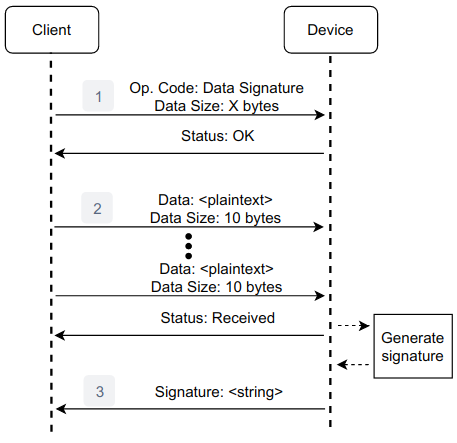
\includegraphics[width=79mm]{Images/signature-generate.png}}
%         \subfigure[Verification]{\label{fig:protocol:signature-verify}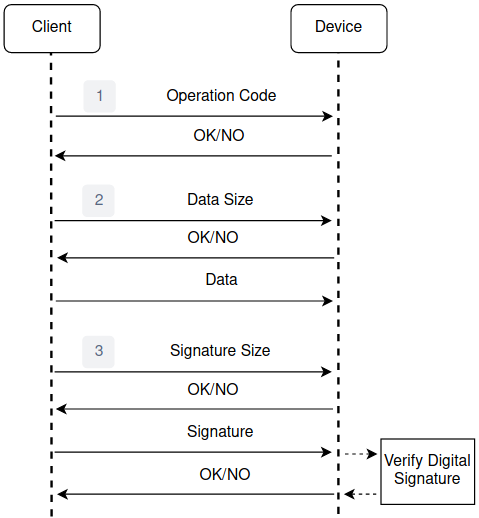
\includegraphics[width=79mm]{Images/signature-verify.png}}
%         \caption{Communication protocol for generating digital signatures and verifying the signatures using the internal HSM asymmetric key pair}
% \end{figure}
\begin{figure}[h!]
	\centering
	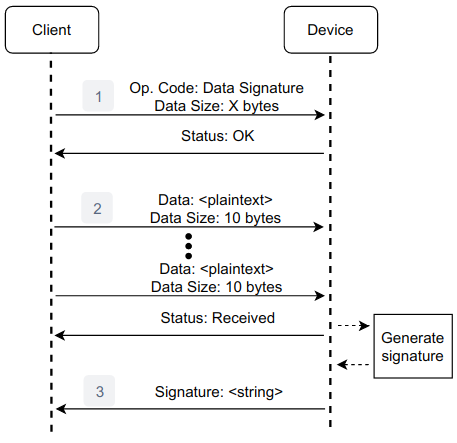
\includegraphics[width=0.55\textwidth]{./Images/signature-generate.png}
	\caption{Communication protocol for generating digital signatures using internal HSM asymmetric key pair}
	\label{fig:protocol:signature-generate}
\end{figure}
The user application sends the operation code, data length and data to be signed.
The qualified digital signature will be generated using the internal private key and data. Afterwards the device responds with the signature length and generated signature.
The device generates the signature with the device's private ECC key, an implementation of the \ac{ECDSA} algorithm and the SHA-256 hash function according to the equation \ref{eq:signature-generate}.

\begin{equation}
	\label{eq:signature-generate}
	Sign_{K}\{Hash\{Data\}\}
\end{equation}

% To verify a signatures, the user sends the operation code, signature length and generated signature, as well as the data length and data from which the signature was generated. The last piece of information sent is the public key of the device, where the signature was generated.
% After verifying the signature, the device responds with the operation status.
% The data is verified using the same hash function, ECDSA algorithm, and the signers' public key, as detailed in \ref{eq:signature-verify}.

% \begin{equation}
%         \label{eq:signature-verify}
%         \{Signature\} == Verify_{K_{-1}}\{Hash\{Data\}\}
% \end{equation}

% -----------------------------------------------------
\subsection{Establishing New Communication Endpoints}\label{chap:arch:services:new-comms}

As introduced before, the device provides the flexibility to establish communications with other entities, even new ones, not previously requested by the user.
The device can also import a new set of keys, provided by the control station.
This way, already established channels of communication can be updated on a regular time schedule.
When a user wants to communicate with a new entity, the system provides two convenient solutions.
Both options allow establishing connections with new entities when needed, by way of a trusted third party: a control station. 
The user can securely contact the control station at any time to request the public key of the other entity, through the secure data exchange service, equivalent to communicating with any other entity. The control station effectively acts as a PKI.
Then, the user sends the information through the computer application to the device. The new key is generated in the device and made available right away. Then data can be exchanged with the new entity, which must also request the control station for the analogous entity's public key.

The system can also be setup with a regular communication update schedule. It grants the flexibility of key revocation when needed, data exchange with new entities, as well as updating symmetric keys, with no additional complexity to the user, to always safeguard the security of communications.
Each month an entity can hand over a list of the entities it wishes to communicate with to the control station, which will accordingly yield the corresponding key set.
Each entity only needs to forward the list to the device, and the new keys are immediately stored and ready to be used.
Users can resume communications, the same way as before with minimal interruption, with the requested entities.
The protocols for both services are detailed next: symmetric key generation and importation of keys.

% -----------------------------------------------------
\subsubsection*{Key Generation}\label{chap:arch:services:new-comms:ecdh}

The protocol to generate a shared symmetric key with another entity, using asymmetric cryptography is detailed in Figure~\ref{fig:protocol:ecdh}.
\begin{figure}[h!]
	\centering
	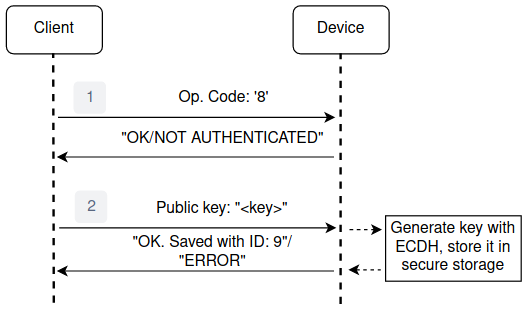
\includegraphics[width=0.60\textwidth]{./Images/ecdh.png}
	\caption{Communication protocol to generate symmetric keys, with an internal private key, to be stored internally}
	\label{fig:protocol:ecdh}
\end{figure}

% The user forwards the operation code, public key and salt value to the device.
The user forwards to the device, the operation code and the public information from the central station: the foreign entity's public key and an additional public salt component.
The generation process depicted in Figure \ref{fig:protocol:ecdh} is thus: first, a secret is computed with the ECDH algorithm, using the device's private key and the received public key. The secret is run through a key derivation function with the salt value, to obtain a new symmetric key.

\begin{equation}
	\label{eq:ecdh-kdf}
	KDF\{ECDH_{K}\{K^{-1}\}, Salt\}
\end{equation}

The same secret can be generated with the device's public key and the foreign entity's private key, in their device. If both entities receive each other's public keys and agree on the same salt value, through the central station, the generated key is identical.
A new unique ID is generated for the key, which is stored in the device, alongside the key. This ID is returned to the user, along with the operation status.
The salt value is used, in order to generate several symmetric keys from the same asymmetric key pairs.

% -----------------------------------------------------
\subsubsection*{Import Keys}\label{chap:arch:services:new-comms:import}

This section details the protocol to import a list of encrypted symmetric keys into the device.
The imported keys must be encrypted with a preset symmetric key, stored inside the device from fabric, using the secure data exchange service. Thus, a central management section with a similar device can distribute keys to the enrolled entities, on a regular schedule.
The protocol for the service is depicted in Figure \ref{fig:protocol:import-keys}.

\begin{figure}[h!]
	\centering
	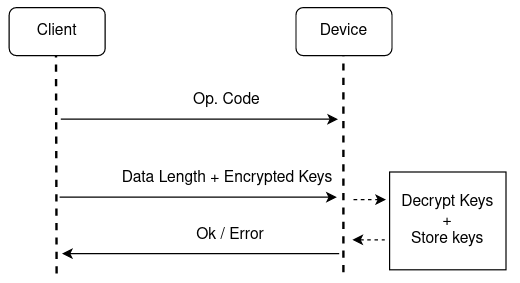
\includegraphics[width=0.60\textwidth]{./Images/import-keys.png}
	\caption{Communication protocol to import encrypted symmetric keys, and store them encrypted in the HSM's non-volatile memory}
	\label{fig:protocol:import-keys}
\end{figure}

The only transmission consists of sending the operation code, key set length and key data. Then, the device decrypts and authenticates the keys using a predefined symmetric key, stored in the device. The protocol used is the same for secure data exchange, as described previously.
Each key data section consists of 1 byte for its ID, 1 byte for its size and remaining bytes for the actual key data.
The decrypted list of keys is encrypted and authenticated again, with a dedicated symmetric key for memory storage. 
The ciphertext, randomly generated IV and ciphertext length are stored in memory. 

To provide authentication and thus protection against tampering, a MAC is generated from the three pieces of data and stored in secure storage, separate from the keys and IV.
In order to fetch a stored symmetric key, the MAC is generated from the key data in memory, and compared to the original. If identical, the keys can be decrypted and a specific key identified through its ID.

% When a symmetric key is revocated, due to reaching its expiration date, or from being compromised, entities can generate a new one, using the aforementioned procedure, with an additional parameter for the key derivation function, to generate a completely new and unique key.
% Import
% Generate

% Supported management operations include generation of new symmetric keys for communication and revocation of existing keys saved in the device, if communications are suspected to be compromised.
% These operations are only available in the scenario where each device has a pair of asymmetric keys, and there is a protocol in place to distribute public keys.

% An entity receives their device, prepared to communicate with other entities, and a list of information of other entities, available to create communications. This information, namely the entities public key, can be imported into the device to generate new keys.
% After the key is imported, a secure connection with a new entity can be established, by sharing symmetric keys.
% In order for an entity to communicate with a another entity, with no previously established communications, their device will generate a new symmetric key and store it in secure storage, or in non-volatile memory, encrypted with the device's public key.

% -----------------------------------------------------
\section{Summary}\label{chap:arch:summary}

This section described the system's functionalities, algorithms and communications protocols, between a secure and portable device, and the user's computer application.
The system grants confidentiality and authentication to communications between any number of users, as soon as they receive the device, without overloading the users with convoluted tasks or responsibilities.
It is very flexible, by allowing entities to manage the authorized user's of their devices and with whom they wish to communicate, by offloading the management responsibility to a trusted control station.
